\documentclass[tikz,border=3pt]{standalone}
\usepackage{pgfplots}
\pgfplotsset{compat=1.18}
\begin{document}
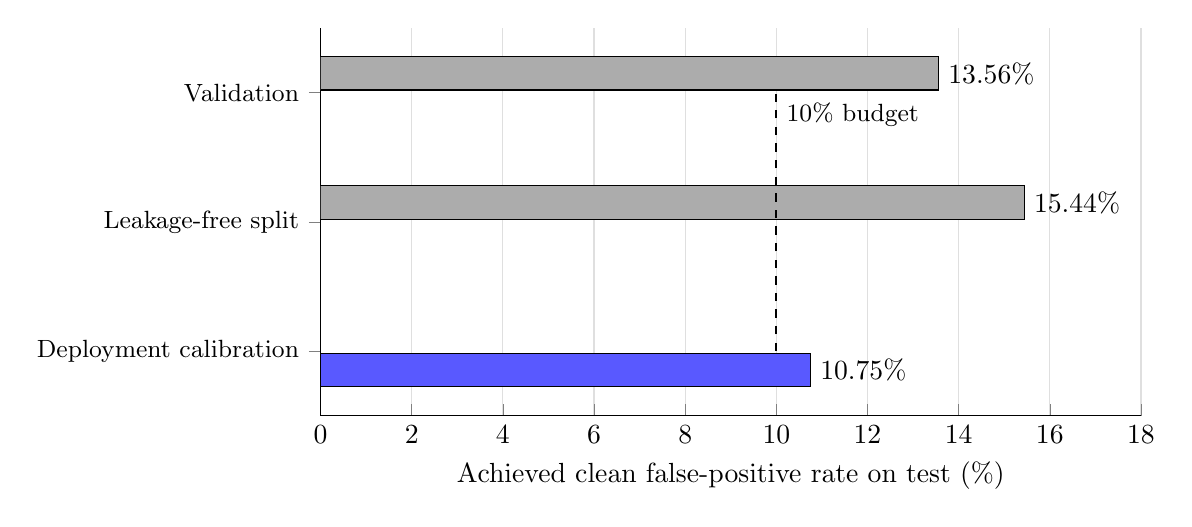
\begin{tikzpicture}
\begin{axis}[
  xbar, width=12cm, height=6.5cm,
  xmin=0, xmax=18,
  xlabel={Achieved clean false-positive rate on test (\%)},
  symbolic y coords={Deployment calibration,Leakage-free split,Validation},
  ytick={Deployment calibration,Leakage-free split,Validation},
  yticklabel style={font=\small},
  enlarge y limits=0.25,
  point meta=x,
  nodes near coords={\pgfmathprintnumber[fixed,precision=2]{\pgfplotspointmeta}\%},
  nodes near coords align={horizontal},
  bar width=12pt,
  axis x line*=bottom, axis y line*=left,
  xmajorgrids=true, grid style={gray!25},
]
\addplot[fill=blue!65] coordinates {(10.75,Deployment calibration)};
\addplot[fill=gray!65] coordinates {(15.44,Leakage-free split) (13.56,Validation)};
\draw[dashed,thick] (axis cs:10,Deployment calibration) -- (axis cs:10,Validation)
 node[pos=1,below right,font=\small]{10\% budget};
\end{axis}
\end{tikzpicture}
\end{document}
